\section{Restricted Boltzmann Machines}\label{sec:rbm}



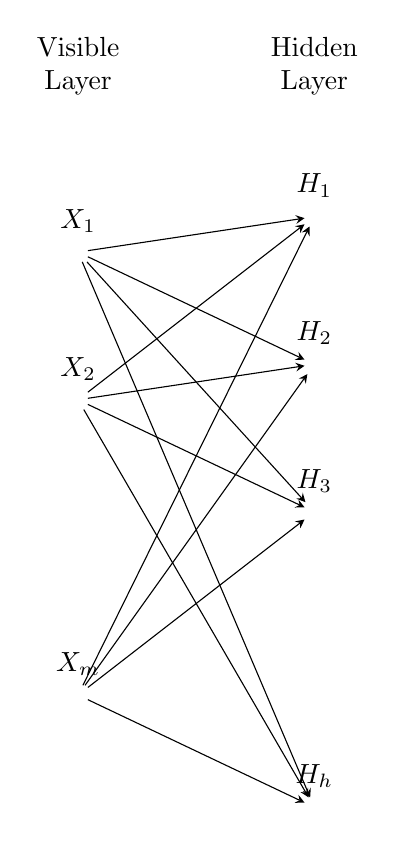
\begin{tikzpicture}[x=1.5cm, y=1.5cm, >=stealth]

\foreach \m [count=\y] in {1,2,missing,3}
	\node [every neuron/.try, neuron \m/.try ] (visible-\m) at (0,2-\y*1.25) {};

\foreach \m [count=\y] in {1,2,3,missing,4}
	\node [every neuron/.try, neuron \m/.try ] (hidden-\m) at (2,2.3-\y*1.25) {};

%this part is only for subscribing nodes , and formatting
\foreach \l [count=\i] in {1,2,...,2,m}
	\node [above] at (visible-\i.north) {$X_{\l}$};
\foreach \l [count=\i] in {1,2,3,...,3,h}
	\node [above] at (hidden-\i.north) {$H_{\l}$};
%drawing part

\foreach \i in {1,...,3}
	\foreach \j in {1,...,4}
		\draw [->] (visible-\i) -- (hidden-\j);

\foreach \l [count=\x from 0] in {Visible, Hidden}
	\node [align=center, above] at (\x*2,2) {\l \\ Layer};

\end{tikzpicture}